\subsection{Solution}
\begin{enumerate}
    \item \textbf{Methods:}
    
    This question can be approached by iterating through the array and finding all possible pairs that sum up to the target.
    
    \item \textbf{Approach:}
    
    \begin{enumerate}
        \item \textbf{Main Function:}
        
        \begin{itemize}
            \item Variables:
            
            \begin{itemize}
                \item \(n\): number of elements in the array
                \item \(array[]\): array that stores the elements
                \item \(target\): the target number that the elements should add up to
            \end{itemize}
            
            \item Method:
            
            \begin{itemize}
                \item Prompt the user to enter the number of elements and the elements themselves.
                \item Validate that all entered numbers are natural numbers.
                \item Ask for the target number.
                \item Iterate through the array to find pairs that sum up to the target.
            \end{itemize}
        \end{itemize}
        
        \item \textbf{generateCombinations Function:}
        
        \begin{itemize}
            \item Variables:
            
            \begin{itemize}
                \item \(arr[]\): array containing the elements
                \item \(data[]\): array to store the combination of indices
                \item \(start\), \(end\): indices to iterate through the array
                \item \(index\): index at which the new index has to be stored
                \item \(r\): size of combinations to generate
                \item \(tar\): target number
            \end{itemize}
            
            \item Method:
            
            \begin{itemize}
                \item Initialize an array with the given size.
                \item Iterate through the array to generate combinations using recursion.
            \end{itemize}
        \end{itemize}
        
        \item \textbf{printCombinations Function:}
        
        \begin{itemize}
            \item Method:
            
            \begin{itemize}
                \item Recursively generate combinations and print those which sum up to the target.
            \end{itemize}
        \end{itemize}
    \end{enumerate}
    
    \item \textbf{Sample C Code:}
    
\begin{lstlisting}[language=C]
#include<stdio.h>
void printCombination(int arr[], int data[], int start, int end, int index, int r, int tar) 
{
    if (index == r) 
    {
    	int sum = 0;
        for (int i = 0; i < r; ++i)
        	sum = sum + arr[data[i]];
        if(sum == tar)
        {
        	printf("INDEX = ");
			for(int j = 0; j < r; j++)
				printf("%d ", data[j]);
			printf("\n");
        }
        return;
    }
    for (int i = start; i < end && end - i >= r - index; ++i) 
    {
        data[index] = i;
        printCombination(arr, data, i+1, end, index+1, r, tar);
    }
}

void generateCombinations(int arr[], int n, int r, int tar) 
{
    int data[r]; 
    printCombination(arr, data, 0, n, 0, r, tar);
}



int main()
{
    int n, target, status;
	printf("Enter the number of elements that you would like to enter: ");
    scanf("%d", &n);
    int array[n];
    printf("Enter your %d numbers: ", n);
    do 
    {
    	status = 1;
    	for (int i = 0; i < n; i++)
    	scanf("%d", &array[i]);  	
    	for (int i = 0; i < n; i++)
    	{
    		if(array[i] <= 0) 
    		{
    			printf("Enter another set of values, because they should be natural numbers: ");
    			status = 0;
    			break;
    		}
    	}
    }
    while (!status);
    printf("Enter your Target Number: ");
    scanf("%d",&target);    
    for(int i = 1; i < n; i++)
    generateCombinations(array, n, i, target); 
    return 0;
}
\end{lstlisting}
    \item \textbf{Output: }
    \begin{figure}[H]
    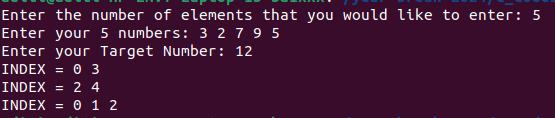
\includegraphics[scale = 0.5]{./figs/two_sum_adv.png}
    \end{figure}
    
\end{enumerate}
